% SCA method, component-level zoom (appendix Figure D.1, fig:method_zoom), TikZ, self-contained.
%
% Build from this directory:  tectonic --outdir .. method_zoom.tex   (writes ../method_zoom.pdf)
% Data and rasters:            fig_method_zoom.py (writes ../method_zoom/{data.tex, block_mask.png,
%                              pi_strip.png} and ../method_zoom_provenance.json; see its docstring)
%
% Same visual language as method.tex: blue = global operator, amber = local,
% green = the calibrated mix, grey = text tokens and structure; titles 9 pt bold
% sans; labels 7 pt sans; single symbols and equations in CM math at 8.5 pt with
% 6.5 pt scripts. Operator drawn: sca_v2 (sca/attn.py, sca_dedup_forward).
%
% (a) Global operator and (b) Local operator are drawn on one toy grid over the
% Figure 1 cathedral (../teaser/square_bright.jpg, the brightened copy used by
% method.tex): H = 24 tokens per side, s = 4, n0 = H / s = 6, t = 2, w = n0 = 6.
% FLUX.1 at 4096^2 has H = 256, s = 4, n0 = 64, t = 8, w = 64 at native steps.
%   (a) block-centre keys kappa(b) = s b + floor(s/2) = 2, 6, ..., 22 (blue dots);
%       one query (dark square, token (13, 9)) and its s x s block; the gathered
%       keys and the query on the coarse n0 x n0 grid of RoPE positions, with the
%       T text keys (grey) that every softmax also sees.
%   (b) query tiles of t x t tokens; the window of tile tau starts at
%       a(tau) = clip(t tau + floor(t/2) - floor(w/2), 0, H - w): an interior tile
%       (tile (3, 4), window cols 4..9, rows 6..11) and a corner tile (11, 11) whose
%       window is clipped from cols/rows 20..25 (dashed) to 18..23. Dotted: the
%       interior tile's window at the widest scheduled side 2 n0 = 12 (cols 1..12,
%       rows 3..14; 128 = 2 x 64 tokens at 4096^2, the first step after the gate).
%       Dark amber dots: the bridge set B, schematic, one token per cell of a 4 x 4
%       grid of 6 x 6-token cells (FLUX.1: 16 tokens per cell of an 8 x 8 grid,
%       1,024 tokens, farthest pre-RoPE keys from the mean key, per block and step),
%       keys of the same softmax at their true positions. The glyph is the block
%       mask of this toy at a native step in tile-major order (rows: 144 query tiles;
%       columns: text keys, bridge keys, then 144 key tiles), ../method_zoom/block_mask.png.
% (c) Gate, ratio lookup and mix: pi_lh(sigma) of block 2, head 8 (one-based) from
%     the scale-2 table (r = 2, dashed) and the scale-4 table (r = 4, solid), linear
%     between the 14 bin centres as in sca/attn.py PiTable. Dots: the weight applied
%     at the 20 post-gate steps; on the four window steps (amber ticks, w = 128, 112,
%     96, 80) it is read at r = 256 / w, log-linear between the tables (table_interp),
%     on native steps from the r = 4 table. sigma > sigma_g = 0.89 is global only
%     (veiled; the effective weight is 0); ticks on the sigma axis are the 28 steps.
% (d) The whole scale-4 table s4_pi_head of src/data/k1_1024_pi.npz: 1368 head
%     columns (57 blocks x 24 heads; heads sorted within each block by the mean of
%     the table at the 20 post-gate step sigmas) by 14 noise bins (sigma 1 at the
%     top to 0 at the bottom; bin 0 is unpopulated and repeats bin 1), raster
%     ../method_zoom/pi_strip.png in the paper-wide pi colormap (scafig.PI_CMAP),
%     with the gate band sigma > sigma_g veiled.

\RequirePackage{fix-cm}
\documentclass[border=0pt]{standalone}
\usepackage[T1]{fontenc}
\usepackage{helvet}
\usepackage{amsmath}
\usepackage{tikz}
\DeclareMathSizes{6.5}{6.5}{6.5}{6.5}
\DeclareMathSizes{7}{7}{6.5}{6.5}
\DeclareMathSizes{8.5}{8.5}{6.5}{6.5}
\usetikzlibrary{arrows.meta, calc}
% Written by scafig.py; the same palette as the matplotlib figures.
\definecolor{scaInk}{HTML}{1F2328}
\definecolor{scaMid}{HTML}{5B6570}
\definecolor{scaRule}{HTML}{C3C9CF}
\definecolor{scaGrid}{HTML}{E6E9EC}
\definecolor{scaGlobal}{HTML}{2F6DB3}
\definecolor{scaGlobalLight}{HTML}{DCE7F3}
\definecolor{scaLocal}{HTML}{E08A2B}
\definecolor{scaLocalLight}{HTML}{F9E6D0}
\definecolor{scaAccent}{HTML}{13865F}
\definecolor{scaAccentLight}{HTML}{D7EEE4}
\definecolor{scaNeutral}{HTML}{F4F1EA}
\definecolor{scaZoom}{HTML}{FFC21A}
\definecolor{scaLoss}{HTML}{B85C00}
\definecolor{scaArea}{HTML}{7A4EA3}
\definecolor{scaAreaLight}{HTML}{E9E0F1}
\definecolor{scaFull}{HTML}{9AA3AC}

\definecolor{piLo}{HTML}{1F4F8A}   % scafig.PI_CMAP end points; the inner stops are
\definecolor{piHi}{HTML}{9C5512}   % scaGlobal (0.22), scaNeutral (0.5), scaLocal (0.78)
% horizontal pi colour bar; TikZ maps 25bp..75bp of a declared shading onto the path
\pgfdeclarehorizontalshading{pibar}{100bp}{color(0bp)=(piLo); color(25bp)=(piLo);
  color(36bp)=(scaGlobal); color(50bp)=(scaNeutral); color(64bp)=(scaLocal);
  color(75bp)=(piHi); color(100bp)=(piHi)}

% inline math inside 7 pt sans labels: CM at 8.5 pt, scripts 6.5 pt
\newcommand{\m}[1]{{\fontsize{8.5}{10}\selectfont$#1$}}

\tikzset{
  every node/.style={inner sep=0pt, outer sep=0pt},
  lbl/.style={font=\sffamily\fontsize{7}{8.4}\selectfont, text=scaInk},
  tick/.style={font=\sffamily\fontsize{6.5}{7.5}\selectfont, text=scaMid},
  ttl/.style={font=\sffamily\bfseries\fontsize{9}{10.8}\selectfont, text=scaInk},
  sym/.style={font=\fontsize{8.5}{10}\selectfont, text=scaInk},
  eq/.style={sym, anchor=base west},
  panel/.style={fill=scaGrid!55, rounded corners=2.5pt},
  flow/.style={->, >={Stealth[round, length=3.5pt, width=3pt]}, draw=scaMid, line width=0.6pt},
  leader/.style={draw=scaMid, line width=0.4pt},
  halo/.style={draw=white, line width=1.1pt},
  blk/.style={rounded corners=2pt, line width=0.8pt},
}

% ---- data written by fig_method_zoom.py from src/data/k1_1024_pi.npz ----
% Written by fig_method_zoom.py from src/data/k1_1024_pi.npz; do not edit by hand.
% panel (b): bridge tokens (x/y, schematic: one per cell of a 4 x 4 cell grid)
\def\bridgedots{3/4,8/4,16/2,19/2,2/8,9/7,14/7,19/7,3/13,9/16,16/15,21/16,1/21,8/21,16/22,19/21}
% panel (c): block 2, head 8 (one-based), centre/pi at r = 2 and r = 4
\def\extwo{0.0357/0.3730,0.1047/0.3730,0.1955/0.3261,0.2748/0.3019,0.3448/0.2862,0.4071/0.2888,0.4627/0.2838,0.5355/0.2898,0.6182/0.3034,0.6873/0.3282,0.7589/0.3659,0.8295/0.4301,0.8955/0.5133,0.9689/0.6395}
\def\exfour{0.0357/0.6776,0.1047/0.6776,0.1955/0.6050,0.2748/0.5740,0.3448/0.5644,0.4071/0.5755,0.4627/0.5842,0.5355/0.6145,0.6182/0.6555,0.6873/0.6999,0.7589/0.7507,0.8295/0.8215,0.8955/0.8980,0.9689/0.9660}
\def\extwolo{0.3730} \def\extwohi{0.6395} \def\exfourlo{0.6776} \def\exfourhi{0.9660}
% weight applied at the 20 post-gate steps: step/sigma/pi/kind (1 = window step, 0 = native step)
\def\applied{9/0.8876/0.5032/1,10/0.8696/0.5552/1,11/0.8504/0.6180/1,12/0.8300/0.6961/1,13/0.8081/0.8001/0,14/0.7847/0.7766/0,15/0.7595/0.7513/0,16/0.7324/0.7319/0,17/0.7031/0.7111/0,18/0.6714/0.6897/0,19/0.6370/0.6675/0,20/0.5994/0.6462/0,21/0.5582/0.6258/0,22/0.5128/0.6051/0,23/0.4627/0.5842/0,24/0.4071/0.5755/0,25/0.3448/0.5644/0,26/0.2748/0.5740/0,27/0.1955/0.6050/0,28/0.1047/0.6776/0}
\def\readsigma{0.4627} \def\readpi{0.5842}
% the 28 sampling sigmas (FLUX.1 shifted schedule, mu = 1.15)
\def\steps{1.0000,0.9884,0.9762,0.9634,0.9499,0.9356,0.9205,0.9045,0.8876,0.8696,0.8504,0.8300,0.8081,0.7847,0.7595,0.7324,0.7031,0.6714,0.6370,0.5994,0.5582,0.5128,0.4627,0.4071,0.3448,0.2748,0.1955,0.1047}


\begin{document}
\begin{tikzpicture}[x=1cm, y=1cm]

% ---------------------------------------------------------------- geometry
\def\W{13.97}      % 5.5 in
\def\Ytop{9.4}     % total height
\def\Yd{3.85}      % top of panel (d)
\def\Yt{3.97}      % bottom of the top row
\def\PW{4.5767}    % top-row panel width, gaps 0.12
\def\Xb{4.6967}
\def\Xc{9.3933}
\path[panel] (0,\Yt) rectangle (\PW,\Ytop);
\path[panel] (\Xb,\Yt) rectangle (\Xb+\PW,\Ytop);
\path[panel] (\Xc,\Yt) rectangle (\W,\Ytop);
\path[panel] (0,0) rectangle (\W,\Yd);

% toy grid shared by (a) and (b): H = 24, s = 4, n0 = w = 6, t = 2
\def\G{2.5}  \def\gt{8.78}   % side and top edge (cm)
\pgfmathsetmacro{\gy}{\gt-\G}
\pgfmathsetmacro{\tc}{\G/24}
\def\ea{5.75} \def\eb{5.3} \def\ec{4.85} \def\ed{4.4}   % equation baselines

% ================================================================ (a) global
\node[ttl, anchor=north west] at (0.18, \Ytop-0.17) {(a) Global operator};
\def\gx{0.2}
\node[anchor=south west] at (\gx,\gy) {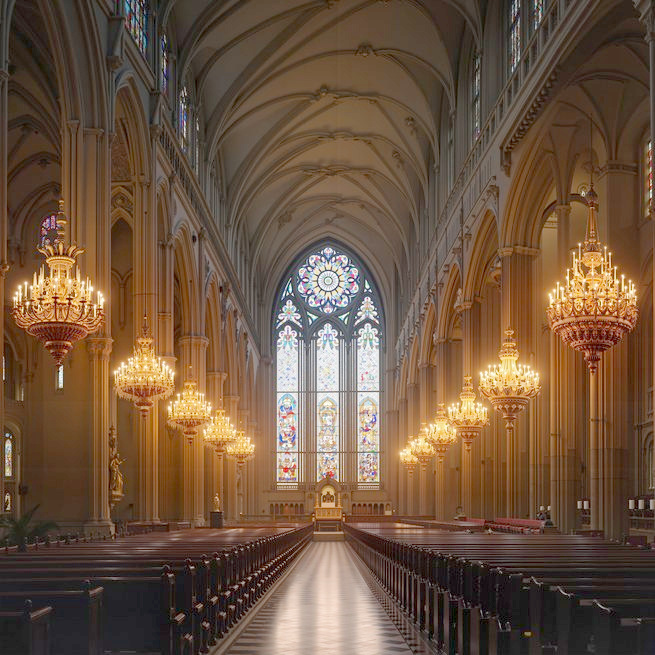
\includegraphics[width=\G cm]{../teaser/square_bright.jpg}};
\begin{scope}[shift={(\gx,\gt)}, x=\tc cm, y=-\tc cm]   % token (i, j), j down
  \foreach \i in {1,...,23} \draw[white, opacity=0.35, line width=0.2pt] (\i,0) -- (\i,24) (0,\i) -- (24,\i);
  \foreach \i in {4,8,...,20} \draw[white, opacity=0.9, line width=0.5pt] (\i,0) -- (\i,24) (0,\i) -- (24,\i);
  \draw[scaGlobal, line width=0.8pt] (12,8) rectangle (16,12);          % the query's s x s block
  \foreach \i in {2,6,...,22} \foreach \j in {2,6,...,22} {
    \fill[white] (\i+0.5,\j+0.5) circle (0.46);
    \fill[scaGlobal] (\i+0.5,\j+0.5) circle (0.33);
  }
  \fill[white] (12.8,8.8) rectangle (14.2,10.2);
  \fill[scaInk] (13,9) rectangle (14,10);                                % query i
\end{scope}
% coarse n0 x n0 grid of RoPE positions: keys at b, the query at c(p_i)
\def\cx{3.2} \def\cs{1.2}
\pgfmathsetmacro{\cy}{\gt-\G+0.62}
\fill[white] (\cx,\cy) rectangle ++(\cs,\cs);
\draw[scaRule, line width=0.3pt] (\cx,\cy) grid[step=0.2] ++(\cs,\cs);
\fill[scaInk] (\cx+0.6,\cy+0.6) rectangle ++(0.2,0.2);
\foreach \i in {0,...,5} \foreach \j in {0,...,5} {
  \fill[white] (\cx+0.1+0.2*\i,\cy+0.1+0.2*\j) circle (0.062);
  \fill[scaGlobal] (\cx+0.1+0.2*\i,\cy+0.1+0.2*\j) circle (0.044);
}
\draw[scaMid, line width=0.4pt] (\cx,\cy) rectangle ++(\cs,\cs);
% text keys, all at position 0
\pgfmathsetmacro{\ty}{\cy+\cs+0.12}
\foreach \i in {0,...,5} \fill[scaMid!80] (\cx+0.2*\i+0.015,\ty) rectangle ++(0.17,0.17);
\node[sym, anchor=east] at (\cx-0.07, \ty+0.085) {$T$};
\node[sym, anchor=south] at (\cx+0.5*\cs, \ty+0.27) {$\mathcal{K}^{\mathrm{glob}}$};
\draw[flow] (\gx+\G+0.08, \cy+0.7) -- (\cx-0.08, \cy+0.7);
% equations
\node[eq] at (0.2, \ea) {$\kappa(b) = s\,b + \lfloor s/2\rfloor$};
\node[eq] at (0.2, \eb) {$c(p_i) = \lfloor p_i/s\rfloor$};
\node[eq] at (0.2, \ec) {$O_i^{\mathrm{glob}} = \mathcal{A}\bigl(q_i,\, c(p_i);\, \mathcal{K}^{\mathrm{glob}}\bigr)$};
\node[eq] at (0.2, \ed) {$|\mathcal{K}^{\mathrm{glob}}| = T + n_0^2$};

% ================================================================ (b) local
\node[ttl, anchor=north west] at (\Xb+0.18, \Ytop-0.17) {(b) Local operator};
\def\hx{4.8967}  % \Xb + 0.2
\node[anchor=south west] at (\hx,\gy) {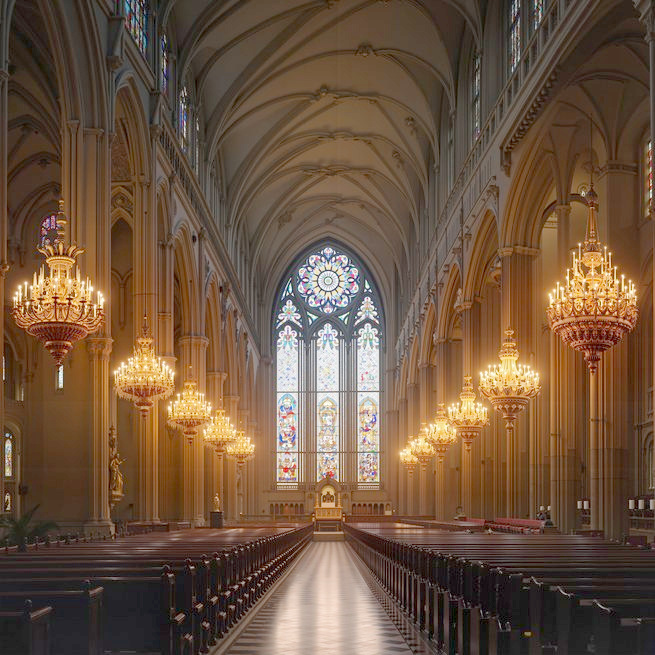
\includegraphics[width=\G cm]{../teaser/square_bright.jpg}};
\begin{scope}[shift={(\hx,\gt)}, x=\tc cm, y=-\tc cm]
  \foreach \i in {1,...,23} \draw[white, opacity=0.3, line width=0.2pt] (\i,0) -- (\i,24) (0,\i) -- (24,\i);
  \foreach \i in {2,4,...,22} \draw[white, opacity=0.75, line width=0.35pt] (\i,0) -- (\i,24) (0,\i) -- (24,\i);
  % interior tile (3, 4) at the widest scheduled side 2 n0 = 12: start (1, 3) (dotted)
  \fill[scaLocal, opacity=0.12] (1,3) rectangle (13,15);
  \draw[white, opacity=0.7, line width=1.1pt] (1,3) rectangle (13,15);
  \draw[scaLocal!85!black, line width=0.8pt, dash pattern=on 1pt off 0.8pt] (1,3) rectangle (13,15);
  \coordinate (wideref) at (1,3);
  % interior tile (3, 4): window starts at a = (4, 6)
  \fill[scaLocal, opacity=0.25] (4,6) rectangle (10,12);
  \draw[scaLocal, line width=0.9pt] (4,6) rectangle (10,12);
  \fill[white] (5.8,7.8) rectangle (8.2,10.2);
  \fill[scaInk] (6,8) rectangle (8,10);
  % corner tile (11, 11): unclamped start a' = 20 (dashed), clipped to a = 18
  \fill[scaLocal, opacity=0.25] (18,18) rectangle (24,24);
  \draw[scaLocal, line width=0.9pt] (18,18) rectangle (24,24);
  \fill[white] (21.8,21.8) rectangle (24,24);
  \fill[scaInk] (22,22) rectangle (24,24);
  \draw[scaLocal, line width=0.6pt, dash pattern=on 1.6pt off 1.2pt] (20,20) rectangle (26,26);
  \coordinate (clipref) at (26,21);
  % bridge set B (schematic): one token per cell of a 4 x 4 cell grid, at its true position
  \foreach \x/\y in \bridgedots {
    \fill[white] (\x+0.5,\y+0.5) circle (0.46);
    \fill[piHi] (\x+0.5,\y+0.5) circle (0.33);
  }
  \fill[white] (5.8,7.8) rectangle (8.2,10.2);
  \fill[scaInk] (6,8) rectangle (8,10);
\end{scope}
\node[sym, anchor=south west, fill=white, inner sep=0.6pt, rounded corners=1pt, text=scaLocal!80!black]
  at ($(\hx,\gt)+(1*\tc,-3*\tc)+(0.02,0.04)$) {$2n_0$};
% the exact block mask, tile-major order
\def\mx{7.8967} \def\mw{1.2}
\node[anchor=north west] (mask) at (\mx, \gt) {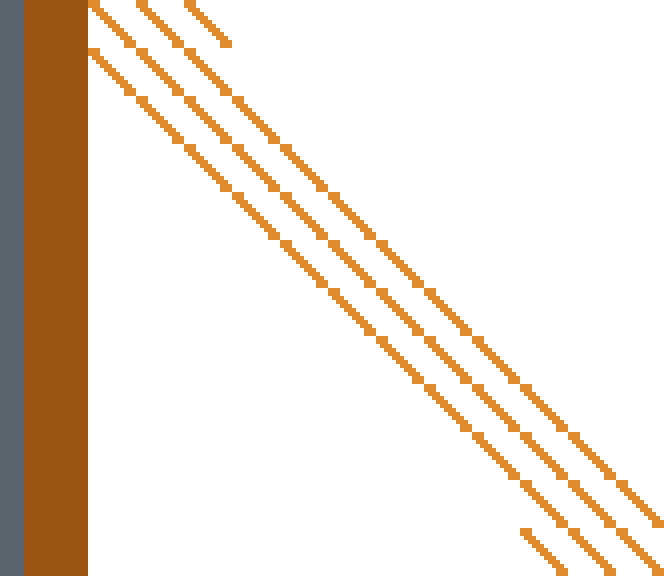
\includegraphics[width=\mw cm]{../method_zoom/block_mask.png}};
\draw[scaMid, line width=0.4pt] (mask.south west) rectangle (mask.north east);
\node[lbl, anchor=north] at ($(mask.south)+(0,-0.08)$) {block mask};
\node[sym, anchor=south] at ($(mask.north west)+(22/166*\mw/2+6/166*\mw/2,0.05)$) {$\mathcal{B}$};
\draw[leader] ($(clipref)+(0.06,0)$) -- (\mx-0.06, \gt-21*\tc);
\node[lbl, anchor=west, text=scaLocal!80!black] at (\mx-0.02, \gt-21*\tc) {clipped};
% equations
\node[eq] at (\Xb+0.2, \ea) {$a' = t\tau + \lfloor t/2\rfloor - \lfloor w/2\rfloor$};
\node[eq] at (\Xb+0.2, \eb) {$a(\tau) = \operatorname{clip}(a',\, 0,\, H - w)$};
\node[eq] at (\Xb+0.2, \ec) {$O_i^{\mathrm{loc}} = \mathcal{A}\bigl(q_i,\, p_i;\, \mathcal{K}_i^{\mathrm{loc}}\bigr)$};
\node[eq] at (\Xb+0.2, \ed) {$|\mathcal{K}_i^{\mathrm{loc}}| = T + |\mathcal{B}| + w(\sigma)^2$};

% ================================================================ (c) gate and mix
\node[ttl, anchor=north west] at (\Xc+0.18, \Ytop-0.17) {(c) Gate and mix};
\def\px{10.0133} \def\pw{3.7} \def\py{7.62} \def\ph{1.05}   % \px = \Xc + 0.62
\def\sg{0.89}
\pgfmathsetmacro{\xg}{\px+(1-\sg)*\pw}
% the example head's two tables, sigma = 0 to 1: flat beyond the outer centres, linear between them
\draw[scaAccent!45, line width=0.7pt, line join=round, dash pattern=on 2pt off 1.2pt]
  (\px+\pw, \py+\extwolo*\ph)
  \foreach \c/\p in \extwo { -- ({\px+(1-\c)*\pw}, {\py+\p*\ph}) }
  -- (\px, \py+\extwohi*\ph);
\draw[scaAccent!45, line width=0.7pt, line join=round]
  (\px+\pw, \py+\exfourlo*\ph)
  \foreach \c/\p in \exfour { -- ({\px+(1-\c)*\pw}, {\py+\p*\ph}) }
  -- (\px, \py+\exfourhi*\ph);
\node[sym, anchor=south east, text=scaAccent] at (\px+\pw, {\py+\exfourlo*\ph+0.05}) {$r{=}4$};
\node[sym, anchor=north east, text=scaAccent] at (\px+\pw, {\py+\extwolo*\ph-0.05}) {$r{=}2$};
% the weight applied at each post-gate step (line): window steps (dots) read at r = 256 / w between the two
% tables, native steps on the r = 4 table
\draw[scaAccent, line width=0.7pt, line join=round]
  \foreach \k/\s/\p/\kind [count=\n] in \applied { \ifnum\n=1 \else -- \fi ({\px+(1-\s)*\pw}, {\py+\p*\ph}) };
\foreach \k/\s/\p/\kind in \applied { \ifnum\kind=1
  \fill[white] ({\px+(1-\s)*\pw}, {\py+\p*\ph}) circle (0.055);
  \fill[scaAccent] ({\px+(1-\s)*\pw}, {\py+\p*\ph}) circle (0.038);
\fi }
% gate: global only above sigma_g
\fill[white, opacity=0.65] (\px,\py) rectangle (\xg,\py+\ph);
\draw[scaGlobal, line width=1.2pt] (\px,\py) -- (\xg,\py);
\draw[scaInk, line width=0.5pt, dash pattern=on 1.6pt off 1.2pt] (\xg,\py) -- (\xg,\py+\ph);
% axes and the 28 sampling steps; the four window steps (w > n0) in amber
\draw[scaMid, line width=0.4pt] (\px,\py+\ph) -- (\px,\py) -- (\px+\pw,\py);
\foreach \s in \steps { \draw[scaMid, line width=0.3pt] ({\px+(1-\s)*\pw}, \py) -- ++(0,0.07); }
\foreach \k/\s/\p/\kind in \applied { \ifnum\kind=1 \draw[scaLocal, line width=0.6pt] ({\px+(1-\s)*\pw}, \py) -- ++(0,0.11); \fi }
\node[tick, anchor=east] at (\px-0.07, \py) {0};
\node[tick, anchor=east] at (\px-0.07, \py+\ph) {1};
\node[sym, anchor=east] at (\px-0.24, \py+0.5*\ph) {$\pi_{lh}$};
\node[tick, anchor=north] at (\px, \py-0.08) {1};
\node[sym, anchor=north] at (\xg, \py-0.08) {$\sigma_g$};
\node[tick, anchor=north] at (\px+\pw, \py-0.08) {0};
\node[sym, anchor=north] at (\px+0.3*\pw, \py-0.08) {$\sigma$};
% the current step reads pi from the table and feeds the mix
\pgfmathsetmacro{\xc}{\px+(1-\readsigma)*\pw}
\pgfmathsetmacro{\yc}{\py+\readpi*\ph}
\draw[scaAccent, line width=0.4pt, dash pattern=on 1pt off 1pt] (\xc,\py) -- (\xc,\yc);
\fill[white] (\xc,\yc) circle (0.065);
\fill[scaAccent] (\xc,\yc) circle (0.045);
% mix: O^glob from the left, O^loc from below, pi from the table above
\pgfmathsetmacro{\ym}{6.2}
\node[blk, sym, draw=scaGlobal, fill=scaGlobal!20, minimum width=1.05cm, minimum height=0.53cm] (og) at (\Xc+0.85, \ym) {$O_i^{\mathrm{glob}}$};
\node[blk, sym, draw=scaLocal, fill=scaLocal!20, minimum width=1.05cm, minimum height=0.53cm] (ol) at (\Xc+0.85, 5.5) {$O_i^{\mathrm{loc}}$};
\node[circle, draw=scaAccent, fill=scaAccent!20, line width=0.8pt, minimum size=0.34cm] (mx) at (\xc, \ym) {};
\draw[scaAccent, line width=0.8pt] ($(mx.center)+(-0.08,0)$) -- ++(0.16,0) ($(mx.center)+(0,-0.08)$) -- ++(0,0.16);
\draw[flow] (og.east) -- (mx.west) node[sym, midway, above=2.5pt] {$1-\pi_{lh}$};
\draw[flow] (ol.east) -| (mx.south) node[sym, pos=0.75, right=2.5pt] {$\pi_{lh}$};
\draw[flow, draw=scaAccent] (\xc, \py-0.45) -- (mx.north);
\draw[flow] (mx.east) -- ++(0.5,0) node[sym, anchor=west, right=2pt] {$O_i$};
\node[lbl, anchor=base west] at (\Xc+0.3, \ec) {\m{\sigma > \sigma_g}: \m{O_i = O_i^{\mathrm{glob}}}};
\node[lbl, anchor=base west] at (\Xc+0.3, \ed) {text queries: \m{O_i = O_i^{\mathrm{glob}}}};

% ================================================================ (d) table
\node[ttl, anchor=north west] at (0.18, \Yd-0.17) {(d) Calibrated table at $r{=}4$, all 57 blocks};
\def\sx{0.75} \def\sw{12.45} \def\sy{1.0} \def\sh{2.2}
\pgfmathsetmacro{\bw}{\sw/57}
\pgfmathsetmacro{\yg}{\sy+\sg*\sh}
\node[anchor=south west] at (\sx,\sy) {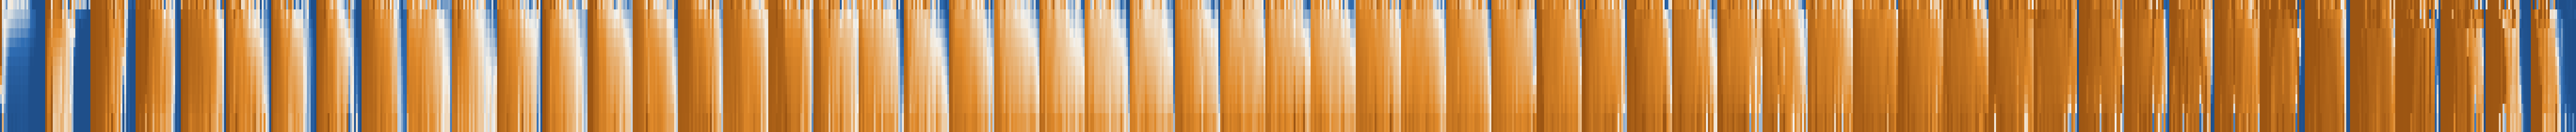
\includegraphics[width=\sw cm, height=\sh cm]{../method_zoom/pi_strip.png}};
\foreach \b in {1,...,56} { \draw[white, opacity=0.7, line width=0.3pt] (\sx+\b*\bw,\sy) -- (\sx+\b*\bw,\sy+\sh); }
\fill[white, opacity=0.6] (\sx,\yg) rectangle (\sx+\sw,\sy+\sh);
\draw[scaMid, line width=0.4pt] (\sx,\sy) rectangle (\sx+\sw,\sy+\sh);
\draw[scaInk, line width=0.5pt, dash pattern=on 1.6pt off 1.2pt] (\sx-0.05,\yg) -- (\sx+\sw+0.05,\yg);
\node[sym, anchor=west] at (\sx+\sw+0.09, \yg) {$\sigma_g$};
\draw[leader] (\sx+36*\bw, 0.5*\yg+0.5*\sy+0.5*\sh) -- (\sx+36*\bw, \sy+\sh+0.16);
\node[lbl, anchor=west] at (\sx+36*\bw+0.06, \sy+\sh+0.19) {global only};
\draw[scaInk, line width=0.8pt] (\sx+19*\bw, \sy-0.05) -- (\sx+19*\bw, \sy+\sh+0.05);
% sigma axis
\node[tick, anchor=east] at (\sx-0.07, \sy+\sh) {1};
\node[tick, anchor=east] at (\sx-0.07, \sy) {0};
\node[sym, anchor=east] at (\sx-0.1, \sy+0.5*\sh) {$\sigma$};
% block axis
\foreach \b in {1,10,20,30,40,50,57} {
  \draw[scaMid, line width=0.4pt] (\sx+\b*\bw-0.5*\bw, \sy) -- ++(0,-0.06);
  \node[tick, anchor=north] at (\sx+\b*\bw-0.5*\bw, \sy-0.1) {\b};
}
\draw[scaMid, line width=0.4pt] (\sx+0.02, 0.56) -- ++(0,0.06) (\sx+0.02, 0.56) -- (\sx+19*\bw-0.04, 0.56) -- ++(0,0.06);
\draw[scaMid, line width=0.4pt] (\sx+19*\bw+0.04, 0.56) -- ++(0,0.06) (\sx+19*\bw+0.04, 0.56) -- (\sx+\sw-0.02, 0.56) -- ++(0,0.06);
\node[lbl, anchor=north] at (\sx+9.5*\bw, 0.48) {double-stream};
\node[lbl, anchor=north] at (\sx+38*\bw, 0.48) {single-stream};
% pi colour bar
\def\cbx{10.9} \def\cbw{2.2} \def\cbh{0.14}
\pgfmathsetmacro{\cby}{\Yd-0.42}
\shade[shading=pibar] (\cbx,\cby) rectangle (\cbx+\cbw,\cby+\cbh);
\draw[scaMid, line width=0.4pt] (\cbx,\cby) rectangle (\cbx+\cbw,\cby+\cbh);
\node[tick, anchor=east] at (\cbx-0.07, \cby+0.5*\cbh) {0};
\node[tick, anchor=west] at (\cbx+\cbw+0.07, \cby+0.5*\cbh) {1};
\node[sym, anchor=east] at (\cbx-0.3, \cby+0.5*\cbh) {$\pi$};

\end{tikzpicture}
\end{document}
